\documentclass[12pt,a4paper]{article}
\usepackage[utf8]{inputenc}
\usepackage[T1]{fontenc}
\usepackage[ngerman]{babel}
\usepackage{csquotes}
\usepackage[backend=biber,style=authoryear,maxcitenames=2,maxbibnames=99]{biblatex}
\addbibresource{Organisation.bib} % Bib-Datei nicht vergessen!
\newcommand{\zitat}[1]{\parencite{#1}}
\usepackage{geometry}
\geometry{
	left=30mm,
	right=30mm,
	top=25mm,
	bottom=25mm
}
\usepackage{graphicx}
\usepackage{float}
\usepackage{setspace}
\onehalfspacing
\usepackage{caption}
\usepackage{tocloft}
\usepackage{hyperref}
\hypersetup{colorlinks=true, linkcolor=black, urlcolor=blue, citecolor=black}
\usepackage{acronym}
\usepackage[nottoc]{tocbibind}
\usepackage{etoolbox} % für robusten Befehl
\usepackage{lipsum} % nur für Blindtext, kann entfernt werden
\usepackage{setspace} % für Zeilenabstand
\usepackage{ragged2e} % für \justifying





\newcommand{\absatzZitat}[1]{%
	\begin{quote}
		\fontsize{10pt}{12pt}\selectfont
		\setstretch{1.0}
		\leftskip=1cm
		\rightskip=1cm
		\justifying
		#1
	\end{quote}
}

\begin{document}
	
	%------------------------- Titelseite -------------------------
	\begin{titlepage}
		\centering
		\vfill
		{\Huge \textbf{Deutsche Telekom}}\\[1.5cm]
		\large
		Seminar: Grundlagen der Organisation\\
		Sommersemester 2025\\[2cm]
		
\includegraphics[width=0.4\textwidth]{images/UOL-Logo.png}\\[2cm]
		\normalsize
		\begin{flushleft}
			\textbf{Betreurin:} Prof. Dr. Julia Brennecke\\[0.5cm]
			\textbf{Abgegeben von:}\\
			Mika Scheinig\\
			Elija Wendte\\
			Justus Kressmann\\
			Engin Fidansoy\\
			Manar Krenbeh\\[0.5cm]
			Carl von Ossietzky Universität Oldenburg\\
			Fakultät II – Informatik, Wirtschafts- und Rechtswissenschaften\\
		\end{flushleft}
		\vfill
		\begin{flushright}
			Abgabedatum: 01. Juni 2025
		\end{flushright}
	\end{titlepage}
	
	%------------------------- Eidesstattliche Erklärung -------------------------
	\pagenumbering{Roman}
	
	\section*{\texorpdfstring{Executive Summary}{Executive Summary }}\label{executive-summary}
	
	In diesem Bericht wird die Aufbau- und Ablauforganisation der Deutschen
	Telekom AG untersucht, die mit rund 200.000 Mitarbeitenden in mehr als
	50 Ländern zu den größten Telekommunikationsanbietern weltweit gehört.
	Der Konzern organisiert sich im Wesentlichen divisional, wobei
	Matrixelemente in Bereichen wie IT, Personal und Strategie hinzukommen.
	Diese hybride Struktur soll Spezialisierung, Kund:innennähe und
	Flexibilität ermöglichen. Allerdings ergeben sich dabei auch
	Schwierigkeiten bei Koordination, Abstimmung und der Bestimmung
	eindeutiger Zuständigkeiten. Die Analyse legt offen, dass interne
	Abläufe teils als schwerfällig wahrgenommen werden.
	Entscheidungsprozesse nehmen viel Zeit in Anspruch, interdisziplinäre
	Kooperation funktioniert nicht optimal, und Silo-Denken erschwert eine
	übergreifende Sichtweise. Agile Arbeitsformen lassen sich unter diesen
	Bedingungen schwer integrieren. Bestehende Initiativen wie digitale
	Lernplattformen, neue Führungsmodelle und bereichsübergreifende Projekte
	sind wichtige Schritte, reichen jedoch nicht aus, um strukturelle
	Schwächen zu beheben.
	
	\noindent Der Schwerpunkt liegt auf der Geschäftseinheit T-Systems, bei der ein
	gesteigerter Veränderungsbedarf festgestellt wurde. Die Analyse zeigt
	Potenziale in Effizienz, Zuständigkeiten und Kulturentwicklung. Erste
	Handlungsideen wie klare Schnittstellen, effizientere Prozesse und
	vernetzte Zusammenarbeit werden skizziert. Der Bericht bildet die Basis
	für einen Folgebericht mit konkreten Empfehlungen zur Reorganisation von
	T-Systems.
	
	
	%------------------------- Inhaltsverzeichnis -------------------------
	\newpage
	\tableofcontents
	\newpage
	
	%------------------------- Abbildungsverzeichnis -------------------------
	\listoffigures
	\newpage
	
	%------------------------- Tabellenverzeichnis -------------------------
	\listoftables
	\newpage
	
	%------------------------- Abkürzungsverzeichnis -------------------------
	\section*{Abkürzungsverzeichnis}
	\begin{acronym}[IT]
		\acro{IT}{Informationstechnologie}
		\acro{BWL}{Betriebswirtschaftslehre}
	\end{acronym}
	\newpage
	
	%------------------------- Kapitelstruktur -------------------------
	
	\pagenumbering{arabic}
	\setcounter{page}{1}
	\begin{center}
		\textbf{Report 1 – Deutsche Telekom}
	\end{center}
	
	
	
	\section{Einleitung und Unternehmensvorstellung}
	
	\subsection{Kontext und Relevanz}
	Warum wurde diese Organisationseinheit gewählt?
	
	Einordnung in das Unternehmen (z.B. Bereich, Funktion, strategische Bedeutung)
	
	\subsection{ Überblick zur Organisationseinheit}
	Größe, Struktur, Aufgabenbereich
	
	Rolle innerhalb des Gesamtunternehmens
	\subsection{Kontext und Relevanz}
	Was soll mit dem Bericht erreicht werden?
	
	Kurze Vorschau auf den inhaltlichen Aufbau
	
	\subsection{Zielsetzung der Analyse}
	Was soll mit dem Bericht erreicht werden?
	
	Kurze Vorschau auf den inhaltlichen Aufbau
	
	
	\section{Analyse der informellen Organisation}
	\subsection{Informelle Strukturen und kulturelle Merkmale}
	Werte, Normen, interne Denkweisen
	
	Machtverhältnisse, Netzwerkstrukturen
	
	Informelle Kommunikation und Entscheidungswege
	\subsection{Elemente moderner Organisationsformen}
	Einsatz von agilen Methoden, selbstorganisierten Teams etc.
	
	Technologische Infrastruktur (z.B. Tools, Plattformen)
	
	Zusammenarbeit über Bereichsgrenzen hinweg (Cross-Functional Work)
	\subsection{Identifizierte Herausforderungen}
	
	Welche Spannungen oder Schwächen ergeben sich aus der Analyse?
	
	Konkrete Pain Points mit Bezug zur Organisationseinheit
	
	Bezug zur Risikoanalyse aus dem Geschäftsbericht
	
\section{Konzeptentwicklung für organisationalen Wandel}

\subsection{Ausgangspunkt und Problemfokus}

Wie in der Analyse gezeigt, stellt die eingeschränkte organisationale Agilität einen zentralen Engpass dar. Langwierige Entscheidungsprozesse, mangelnde bereichsübergreifende Abstimmung und eine begrenzte Reaktionsfähigkeit erschweren die Zusammenarbeit und mindern die Innovationskraft der Organisation.

\noindent Das folgende Konzept greift diesen Pain Point gezielt auf und verbindet technologische mit organisatorischen Hebeln, um Entscheidungswege zu verkürzen und Strukturen anpassungsfähiger zu gestalten. Im Fokus stehen vier ineinandergreifende Wirkfelder: der Einsatz von Cloud- und SaaS-Technologien, der Ausbau datenbasierter Entscheidungsunterstützung (BI), die Stärkung bereichsübergreifender HR- und Wissensprozesse sowie die Einführung agiler Organisationsformen. Die Maßnahmen orientieren sich an den im Geschäftsbericht 2021 genannten Risikofeldern und zielen auf eine robuste, flexible und skalierbare Entscheidungsarchitektur ab.



	
\subsection{Zielsetzung des Konzepts}

Das übergeordnete Ziel des vorliegenden Konzepts besteht darin, die organisationale Agilität innerhalb der betrachteten Organisationseinheit der Deutschen Telekom gezielt zu stärken. Hierzu sollen strukturelle, technologische und kulturelle Voraussetzungen geschaffen werden, die eine schnellere, koordinierte und flexiblere Reaktion auf externe Anforderungen ermöglichen.

\noindent Die Zielsetzung folgt dem in der strategischen Zielplanung etablierten System aus Sach- und Formalzielen \parencite{StelzerDirk1962-2011I:GA}. Im Zentrum stehen folgende Zielinhalte:

\begin{itemize}
	\item \textbf{Sachziel:} Erhöhung der Anpassungsfähigkeit der Organisation an regulatorische, technologische und marktbezogene Veränderungen durch den gezielten Einsatz agiler Arbeitsformen, cloudbasierter Informationssysteme und strukturierter Wissensprozesse.
	\item \textbf{Formalziele:} Erhöhung der Wirksamkeit durch zentrale Entscheidungen und BI-Transparenz, mehr Anpassungsfähigkeit durch flexible SaaS-Workflows und Teams sowie durch Systemnutzung und schrittweisen Rollout.
\end{itemize}



\subsection{Zielsystem}\label{sec:zielsystem}

\begin{itemize}
	\item \textbf{Ziel 1:} Innerhalb von zwölf Monaten soll die durchschnittliche Dauer bereichsübergreifender Entscheidungsprozesse um mindestens 30\,\% gesenkt werden – gemessen als Zeitspanne zwischen Initiierung und Umsetzung (KPI: Entscheidungsdurchlaufzeit).
	
	\item \textbf{Ziel 2:} Die Zustimmung zur Aussage „Veränderungen werden nachvollziehbar kommuniziert“ soll nach sechs Monaten mindestens 75\,\% betragen, gemessen über eine interne Zufriedenheitsabfrage (KPI: Change-Kommunikationsfeedback).
\end{itemize}

\subsection{Konzeptionelle Ansätze und Maßnahmen}
\subsubsection{Ansatz 1}
Integriertes Konzept zur agilen Entscheidungsunterstützung: Kombination aus Business Intelligence und SaaS.


\paragraph{1. BI-basierte Entscheidungsunterstützung: Daten als Entscheidungsgrundlage}
Basierend auf den Erkenntnissen von Smith und Ariyachandra (2021) zeigt sich, dass eine einfache, aber gut strukturierte BI-Lösung Entscheidungsprozesse deutlich verbessern kann. Am Beispiel der FEMA-Studie betonen die Autoren:

\begin{quote}
	A simple integrated BI solution [...] can vastly enhance the post disaster operations [...] and improve its agility during humanitarian crises. \parencite[210]{rahman_achieving_2022}.
\end{quote} 


\noindent Die darin beschriebenen Herausforderungen – etwa fehlende Transparenz, lange Entscheidungswege und unklare Zuständigkeiten – lassen sich in ähnlicher Form auch bei der Deutschen Telekom beobachten. 

\noindent Um diese Probleme gezielt anzugehen, empfiehlt sich ein strukturiertes Vorgehen auf Basis folgender fünf Bausteine:

\begin{itemize}
\item \textbf{Datenerfassung und -bereinigung:} Im Fokus stehen operative Daten aus Systemen der Telekom – etwa zu Projekten, IT-Tickets oder Personaleinsätzen. Diese sollen automatisiert validiert und konsolidiert werden, um Entscheidungsgrundlagen zu verbessern. Denn: „Data accuracy and data completeness are […] key problems“ \parencite[S.~201]{rahman_achieving_2022}.


	\item \textbf{Zentrale Datenintegration:} Aufbau eines cloudbasierten, einheitlichen Entscheidungsdatenmodells mit klaren Schnittstellen zwischen den Bereichen.
	\item \textbf{Rollenbasiertes Echtzeit-Reporting:} Dashboards liefern Kennzahlen zu Entscheidungsdauer, Rückläufen und Beteiligung – je nach Rolle.
	\item \textbf{Governance-Struktur:} Einführung klarer Zuständigkeiten für Datenqualität, Reporting und KPI-Management.
	\item \textbf{Pilotierung:} Testlauf mit agilen, interdisziplinären Teams zur schrittweisen Ausweitung und Akzeptanzsicherung.
\end{itemize}

\noindent Ziel ist es, Entscheidungen nachvollziehbarer, schneller und datengestützt zu gestalten – ein zentraler Hebel zur Förderung der Agilität im Unternehmen.
\paragraph{2. SaaS-basierte Entscheidungsstrukturen: Prozesse flexibel gestalten}

Während Business Intelligence (BI) vorrangig auf bessere Entscheidungsgrundlagen abzielt, erweitert der Software-as-a-Service-Ansatz (SaaS) diesen Fokus, indem er die Entscheidungsprozesse selbst flexibler, transparenter und technisch skalierbarer gestaltet. Für einen Konzern wie die Deutsche Telekom bietet SaaS damit die Chance, komplexe Entscheidungswege zu verschlanken, Zuständigkeiten klarer zu strukturieren und Prozesse dynamisch anzupassen.

\noindent Entscheidungsstrukturen lassen sich so als digitale Services abbilden – mit klaren Schnittstellen, automatisiertem Feedback und standardisierter Überwachung. Cloudbasiertes Wissensmanagement kann dabei die nötige Agilität schaffen, um qualitativ hochwertige Entscheidungsprozesse zu unterstützen \parencite{churakova2010software}.


\noindent Die Umsetzung erfolgt idealerweise schrittweise nach einem angepassten Implementierungsmodell von Chou und Chou (2011), das auf den Arbeiten von \parencite{murthy2010tapping}, \parencite{chong2006multi} sowie \parencite{buyya2008market} basiert. Es umfasst sechs aufeinander aufbauende Phasen und wurde speziell für komplexe SaaS-Migrationen in großen Organisationen angepasst (vgl. Abbildung~\ref{fig:saas-implementation-plan}).



\begin{figure}[H]
	\centering
	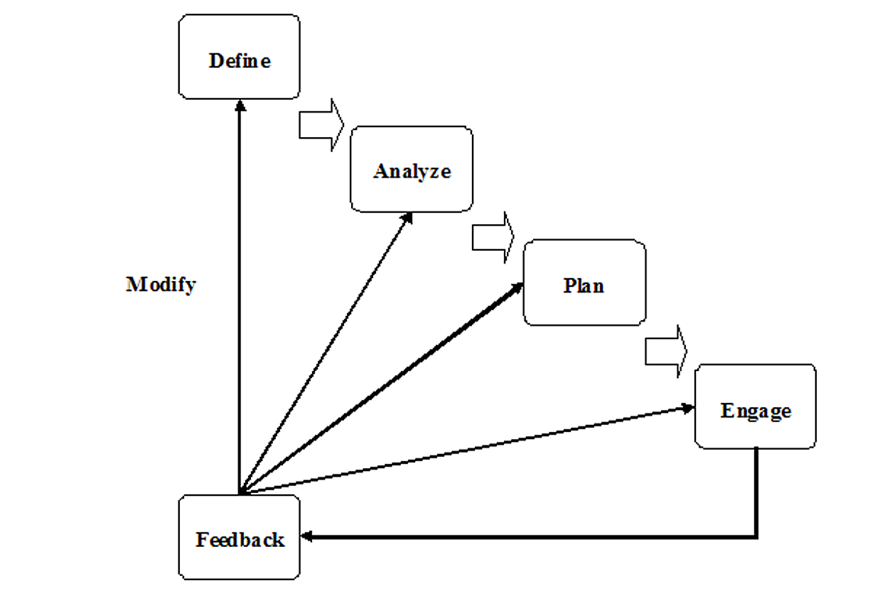
\includegraphics[width=0.6\textwidth]{./images/saas_implementation_plan.png}
\caption{Modifizierter SaaS-Implementierungsplan nach \textcite{chou2011cloud}, basierend auf \textcite{murthy2010tapping}, \textcite{chong2006multi} und \textcite{buyya2008market}}
	\label{fig:saas-implementation-plan}
\end{figure}

\begin{itemize}
	\item \textbf{Define:} Zu Beginn steht die klare Definition bestehender Schwachstellen, z.\,B. Medienbrüche, unklare Verantwortlichkeiten oder isolierte Systeme.
	\item \textbf{Analyze:} Es folgt eine Analyse der bestehenden IT-Struktur, der Ziele der jeweiligen Fachbereiche sowie möglicher Integrationshürden.
	
	\item \textbf{Plan:} Auf dieser Basis wird die SaaS-Migration geplant. Dazu gehört die Auswahl passender Anbieter, die Festlegung technischer Anforderungen und die Klärung rechtlicher Rahmenbedingungen (z.\,B. Datenschutz, SLAs).
	
	\item \textbf{Engage:} Die Umsetzung beginnt zunächst in kleineren Einheiten (z.\,B. einem Bereich mit hoher Abstimmungsintensität), um schnell Erfahrungen zu sammeln und Verbesserungen vorzunehmen.
	
	\item \textbf{Feedback:} Erste Umsetzungsschritte werden kontinuierlich evaluiert – etwa im Hinblick auf Nutzbarkeit, Schnittstellenstabilität oder Akzeptanz bei den Mitarbeitenden.
	
	\item \textbf{Modify:} Auf Basis dieser Rückmeldungen werden technische und organisatorische Anpassungen vorgenommen. Ziel ist eine passgenaue Weiterentwicklung der Lösung mit Blick auf Skalierung.
\end{itemize}

\noindent Die Deutsche Telekom kann mit diesem Ansatz Entscheidungsprozesse serviceorientiert, nachvollziehbar und flexibel gestalten. Das stärkt unmittelbar die definierten Formalziele: Softwaregestützte Strukturen erhöhen die Wirksamkeit, konfigurierbare Workflows verbessern die Anpassungsfähigkeit und zentral nutzbare Dienste steigern die Wirtschaftlichkeit – auch bereichsübergreifend.

\noindent Die Kombination aus BI (für fundierte Entscheidungsinhalte) und SaaS (für anpassbare Strukturen) ergibt ein integriertes Konzept zur Steigerung organisationaler Agilität – als technologische und analytische Antwort auf die Herausforderungen moderner Konzernsteuerung.

\subsubsection{Ansatz 2}
\paragraph{Kontextuelle Ambidexterität als Kulturansatz zur Stärkung der Change-Kommunikation}


Neben technologischen Hebeln erfordert nachhaltige Agilität auch kulturelle Voraussetzungen. Ein vielversprechender Ansatz ist hier die kontextuelle Ambidexterität, bei der Mitarbeitende befähigt werden, selbstständig zwischen Effizienz (Exploitation) und Innovation (Exploration) zu balancieren. Anstatt auf feste Strukturen oder einzelne Führungspersönlichkeiten zu setzen, entsteht ein Umfeld, in dem Entscheidungs- und Anpassungsfähigkeit breit verankert sind.

\noindent\textcite{kumkale_organizational_2022} beschreiben diesen Ansatz als Führung durch Kontext:
\begin{quote}
	Ambidexterity does not come into view from the formal structure alone or the vision statements of a charismatic leader, but rather requires the creation of a supportive context in which individuals make their own choices about how and where to focus their energies. \parencite[18]{kumkale_organizational_2022}.
\end{quote}



\noindent Für die Telekom bedeutet dies, die Voraussetzungen zu schaffen, damit Führung auf allen Ebenen gelebt werden kann – insbesondere in Phasen des Wandels. Dazu zählen:

ein klar formulierter Handlungsrahmen (Alignment),

die aktive Einbindung von Mitarbeitenden in Entscheidungen (Empowerment),

sowie eine Feedbackkultur, die Lernen und Anpassung ermöglicht (Adaptability).

\noindent Ziel ist es, die Zustimmung zur Aussage „Veränderungen werden nachvollziehbar kommuniziert“ nachhaltig zu erhöhen (vgl. Ziel 2 in Abschnitt~\ref{sec:zielsystem}). Die Stärkung von Eigenverantwortung und Orientierung im Alltag fördert nicht nur das Verständnis für Wandel, sondern verbessert auch die Qualität der Umsetzung selbst.
	
	\section{Diskussion der Ergebnisse}
		\subsection{Umgang mit potenziellen Widerständen}
	Bezug auf bekannte Widerstandsursachen (vgl. Abbildung)
	
	Maßnahmen zur Förderung der Akzeptanz:
	
	Partizipation
	
	Change Agents
	
	Kommunikation und Transparenz
	
	Weiterbildung
	
	Ziel: Konzept so gestalten, dass es nicht gegen, sondern mit den Mitarbeitenden umgesetzt wird
	
	\subsection{Voraussetzungen und Erfolgsfaktoren}
	Was braucht es, damit das Konzept funktioniert?
	→ z.B. Unterstützung durch Führung, Ressourcen, Pilotbereiche
	
	Verbindung zu bestehenden Initiativen in der Organisation (z.B. Tech  Innovation bei der Telekom)
	\subsection{Bewertung der vorgeschlagenen Maßnahmen}
	
	Was leisten die Maßnahmen im Hinblick auf die analysierten Probleme?
	Welche Verbesserungen wären zu erwarten?
	\subsection{Potenziale und Chancen}
	Welche Entwicklungsmöglichkeiten ergeben sich für die Organisationseinheit?
	
	Langfristiger Nutzen (z.B. Innovationskraft, Arbeitgeberattraktivität)
	\subsection{Risiken und Grenzen}
	Was könnte die Umsetzung erschweren? (z.B. Ressourcen, Akzeptanz, Führung)
	
	Wo stößt das Konzept an Grenzen?
	
	\subsection{Einschätzung zur Umsetzbarkeit}
	Was spricht für die praktische Umsetzung?
	
	Welche Voraussetzungen müssen erfüllt sein?
	%------------------------- Literaturverzeichnis -------------------------
	
	\newpage
	\pagenumbering{roman}
	\printbibliography[heading=bibintoc,title={Literaturverzeichnis}]
	
	
	%------------------------- unternehmensinfo -------------------------
	\newpage
	\thispagestyle{empty} % keine Seitenzahl anzeigen
	\begin{figure}[H]
		\centering
		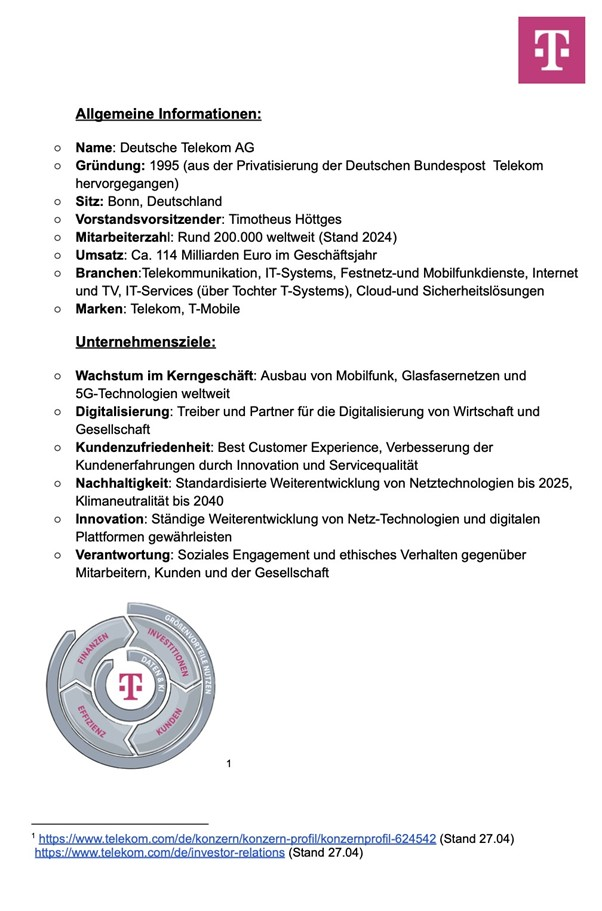
\includegraphics{images/Bild1.jpg}
	\end{figure}
	\newpage
	%------------------------- Anhang -------------------------
	\newpage
	\section{Anhang}
	[Zusätzliche Materialien wie Interviewleitfäden etc.]
	
	%------------------------- KI-Nutzung -------------------------
	\newpage
	\section{Anhang: Nutzung von Künstlicher Intelligenz}
	\begin{itemize}
		\item \textbf{Tool:} ChatGPT
		\item \textbf{URL:} \url{https://chatgpt.com}
		\item \textbf{Prompt:} „Erstelle eine vollständige LaTeX-Vorlage für eine Gruppenarbeit.“
		\item \textbf{Verwendet durch:} Manar Krenbeh
		\item \textbf{Datum:} 04.07.2025
	\end{itemize}
	\begin{itemize}
		\item \textbf{URL:} \url{https://chatgpt.com/share/682f2a68-37b8-8007-9855-d878bcd54ae3}
		\item \textbf{Prompt:} „Kannst du mir ein konkretes Beispiel für einen überregulierten internen Prozess der Deutschen Telekom nennen?“
		\item \textbf{Verwendet durch:} Mika Scheinig
		\item \textbf{Datum:} 22.05.2025
	\end{itemize}
	
	\begin{itemize}
		\item \textbf{URL:} \url{https://chatgpt.com/c/683721e2-4a9c-8001-b0a1-f2e5a1b3f5f2}
		\item \textbf{Prompt:} „Bitte erläutere die Unterschiede in der Leitungsspanne zwischen standardisierten operativen Bereichen und komplexeren Organisationseinheiten wie der Matrixorganisation bei T-Systems. Wie beeinflusst die Organisationsstruktur die Anzahl der direkt unterstellten Mitarbeitenden, und welche Herausforderungen ergeben sich für Führungskräfte in einer Matrixstruktur?“
		\item \textbf{Verwendet durch:} Justus Kressmann
		\item \textbf{Datum:} 24.05.2025
		\item \textbf{Tool:} NoteBookml
		\item \textbf{URL:} \url{https://notebooklm.google.com}
		\item \textbf{Prompt:} "Finde aus dem Buch konkrete Methoden, wie Informationssysteme genutzt werden können, um Entscheidungsprozesse in Organisationen zu beschleunigen oder transparenter zu machen. Bitte nenne die jeweiligen Kapitel oder Autorenbeiträge." Hier \parencite{StelzerDirk1962-2011I:GA} verwendet
		\item \textbf{Verwendet durch:} Manar Krenbeh
		\item \textbf{Datum:} 05.07.2025
		\item \textbf{Prompt:} "Suche im Buch nach alternativen Lösungsansätzen oder Methoden zur Verbesserung der internen Kommunikation von Veränderungen im Unternehmen – ohne Bezug auf SaaS oder Business Intelligence." Hier \parencite{kumkale_organizational_2022} verwendet
		\item \textbf{Verwendet durch:} Manar Krenbeh
		\item \textbf{Datum:} 05.07.2025
	\end{itemize}
	
	\newpage
	\section*{Eidesstattliche Erklärung}
	Hiermit versichern wir, dass wir die vorliegende Arbeit selbstständig und nur mit den angegebenen Hilfsmitteln und Quellen angefertigt haben. Alle Stellen, die wörtlich oder sinngemäß aus Quellen übernommen wurden, sind entsprechend kenntlich gemacht. Die Arbeit wurde in gemeinsamer Verantwortung erstellt.
	
	\vspace{2cm}
	Oldenburg, 01. Juni 2025
	
	Unterschriften: \\
	\rule{5cm}{0.4pt} Mika Scheinig \\
	\rule{5cm}{0.4pt} Elija Wendte \\
	\rule{5cm}{0.4pt} Justus Kressmann \\
	\rule{5cm}{0.4pt} Engin Fidansoy \\
	\rule{5cm}{0.4pt} Manar Krenbeh
	
\end{document}
